\section{Introduction to Blockchain}
\subsection{What is Blockchain}
From a technical point of view, Blockchain is a distributed ledger that is cryptographically
secure, append-only, immutable (extremely hard to change), and updateable only
via consensus among nodes.

From a business point of view, a blockchain can be defined as a platform
whereby peers can exchange values without the need for a central trusted party
by using transactions which are stored inside the blockchain in a verifiable and
permanent way.












\subsection{Blockchain features}

\subsubsection*{Decentralization}
This is the core feature of Blockchain. Thanks to decentralization there's no
need of a central trusted entity which stores the data and validates the
transaction, since the same copy of the Blockchain is stored by every node and
the validation of transaction is achieved through consensus.

\subsubsection*{Distributed consensus}
Blockchain have a high Byzantine Fault Tolerance\footnote{without BFT, a peer
would able to transmit and post false transactions} and allows to achieve
distributed consensus, therefore allows to have a single version of a data value
agreed by all parties without requiring a central authority.

\subsubsection*{High availability}
Blockchain is based on a peer-to-peer network of thousands of nodes and data is
replicated on each node, therefore the whole system is highly available since even
if one or more nodes fail the whole network can continue to work correctly.


\subsubsection*{Immutability}
All the data stored in a blockchain is immutable: once a block has been added to
the blockchain, it is considered pratically impossible to change it (changing it
is computationally infeasible since it would require an unaffordable amount of
computing resources).

\subsubsection*{Transparency}
Blockchain is shared between the nodes and everyone can see what is in the
blockchain, thus allowing the system to be transparent and trusted.

\subsubsection*{Security}
Blockchain ensures the integrity and the availability of the data. Since
private keys and digital signatures are used, it also provide authentication and
non-repudiation. It doesn't provide confidentiality, due to it's transparency
feature (privacy is however required in certain scenarios, thus research in
this area is being carried out).

Blockchain security is due especially to its distributed nature, since for an
attacker would be a lot easier to tamper with data if it was stored on a single
central entity.

\subsubsection*{Uniqueness}
In Blockchain every transaction is unique and has not been spent already.
This is especially usefull in cryptocurrencies applications of Blockchain,
where avoidance of double spending is a key requirement.















\subsection{Blockchain structure}
As shown in figure \ref{fig:blockchain-basic-schema}, a blockchain consists of
linked list of ordered fixed-length blocks, each of which includes a set of transactions.
In this section, the generic elements of a blockchain will be presented.
\begin{figure}[!htb]
	\centering
	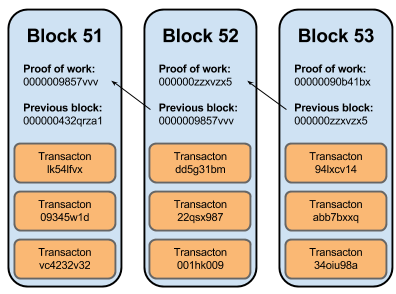
\includegraphics[width=0.5\linewidth]{img/blockchain-basic-schema.png}
	\caption{basic blockchain schema}
	\label{fig:blockchain-basic-schema}
\end{figure}

\subsubsection*{Blocks}
A block groups transactions in order to organize them logically and its size
depends on the blockchain implementation. Generally, a block is composed of:
\begin{itemize}
  \item a set of transactions
  \item a hash which identifies the block
  \item a pointer to the previous block hash (unless it's the genesis block)
  \item a nonce
  \item a timestamp
\end{itemize}
The \emph{genesis block} it's simply the first block in the blockchain and therefore
it can't contain any reference to the previous block.


\subsubsection*{Addresses}
Addresses are unique identifiers which identify the parties involved in a
transaction. An address is usually a public key or it's derived from a public key.


\subsubsection*{Transactions}
A transaction is a tranfer of value from an address to another.


\subsubsection*{Peer-to-peer network}


\subsubsection*{Transaction scripts}
Transaction scripts are predefined sets of commands for nodes to transfer values
from one address to another and perform various other functions.


\subsubsection*{Programming language and Virtual machine}
A Turing-complete programming language is an extension of transaction scripts and
it allows the peers to define the operations that has to be performed on a
transaction, without the limitations of a non-Turing-complete transaction script.
Programs encapsulate the business logic and can for example transfer a value
from one address to another only if some conditions are met.

A virtual machine allows Turing-complete code to be run on a Blockchain as
smart contract (e.g. Ethereum virtual machine).

Not every Blockchain supports Turing-complete programming languages and virtual
machines (e.g. Bitcoin is not Turing-complete\footnote{It however supports
smart contracts}).


\subsubsection*{Nodes}
A node is an active entity which stores a copy of the blockchain and can perform
and/or valide transactions (following a consensus protocol, e.g. the Proof of Work).









\subsection{Consensus in Blockchain}
Consensus in Blockchain is required to establish wheter the ledger itself or
a piece of information submitted to it are valid or not. In analogy with the
Byzantine Generals Problem, the ``generals/lieutenants'' are the nodes partecipating
in the blockchain, the messangers are the network used by the nodes for communicating
and the ``traitors'' are the nodes which try to tamper with the data by submitting
for example false data or by modifying the existing blocks.

In today Blockchain implementations are used four main consensus mechanisms:
the Pratical Byzantine Fault Tolerance (PBFT), the Proof of Work (PoW),
the Proof of Stake (PoS) and the Delegated Proof of Stake (DPoS).

\subsubsection{Practical Byzantine Fault Tolerance Algorithm (PBFT)}
The PBFT is an algorithm proposed by M. Castro and B. Liskov as an optimized solution
to the Byzantine Generals Problem (more in general, it is an efficiet replication
algorithm that is able to tolerate Byzantine faults \cite{castro1999practical}).

Simplifying, the algorithm works as follows \cite{blockchain-consensus-medium},
\cite{castro1999practical}: each ``general'' maintains an
internal state and when he receives a message, he uses the message in
conjunction with his internal state to run a computation, which tells to the
general what to think about the message in question.
After reaching his individual decision about the message, the general shares that
decision with all the other ``generals'' in the system.
A consensus decision is determined based on the total decisions submitted by all
generals.


The advantage of this method is that is very efficient and allows to establish
consensus with less effort than other methods. The main disadvantage is that it
precludes the anonimity of users on the system.

Two example of Blockchains which use PBFT are Hyperledger and Ripple.

\subsubsection{Proof of Work (PoW)}
Contrary to the PBFT, Proof of Work doesn't require all nodes to submit their
individual conclusions in order for a consensus to be reached. Instead, this
mechanism relies on proof that enough computational resources have been spent
before proposing a value for acceptance by the network: only a single node (the first one)
announces its conclusions about the submitted information and those conclusions
can then be independently verified by all other nodes in the system.

This is the consensus scheme used by Bitcoin (see chapter \ref{sec:Bitcoin}).

\subsubsection{Proof of Stake (PoS)}\label{sec:proof-of-stake}
This consensus mechanism is similar to the PoW but in this case the network
selects an individual to confirm the validity of new information submitted to
the ledger based on the nodes' stake in the network. Therefore, instead of any
individual attempting to carry out an intensive computation in order to propose
a value, the network itself runs a lottery based on the nodes' stake to decide
who will announce the results: the more stake one node has, the higher the probability
to be chosen is.

The main idea behind the PoS mechanism is that if a node that has enough stake in
the system it means that it has invested enough in the system so that any
malicious attempt would outweigh the benefits of performing an attack on the
system.

The main problem of this approach is that the system rewards moore those who
already are most deeply involved in the network leading consequently to an
increasingly centralized system.

This mechanism has been adopted by Peercoin.

\subsubsection{Delegated Proof of Stake (DPoS)}
This method is an evolution of the PoS whereby each node that has stake in the
system can choose an entity to represent their portion of stake in the system
by voting. The more stake one node has, the higher is the weight of is vote.
The entity with most votes (weighted) becomes a delegate which validates transactions
(and collects rewards for doing so).
% What if the delegate is incorrect? The nodes stop voting it and change delegate

This method is adopted by Bitshares.

\subsection{Types of Blockchain}
Blockchain can be distinguished into three different types, each one charaterized
by a certain set of attributes.
\subsubsection*{Public Blockchain}
Public Blockchains are blockchains open to the public in which everyone can join
the network, mantain the shared ledger and partecipate in the consensus process.
The ledger is therefore owned by noone and is publicly accessible by everyone.

These type of Blockchain typically have an incentivizing mechanism to encourage
more participants to join the network. Bitcoin for example, one the largest public
Blockchain, reward with cryptocurrency miners who join the network.

Public Blockchains have two main disadvantages: the substantial amount of
computational power required to maintain a distributed ledger at a large scale
and the lack of privacy for the transactions stored inside the blockchain.

\subsubsection*{Private Blockchain}
Private blockchains are private and open only to an organization or a group of
individuals. Participants need to obtain an invitation or permission to join the
Blockchain and mantain the ledger.
Usually the network is permissioned: there are restrictions on who
is allowed to participate in the network, and only in certain transactions.

An example of private blockchain with permissioned network is the Linux
Foundation's Hyperledger Fabric \cite{hyperledger-fabric}.

\subsubsection*{Consortium Blockchain}
Consortium blockchains are blockchains where the consensus process is controlled
by a preselected set of nodes (e.g. a consortium of organization, each of which
operates a node). The right to read the blockchain might be public or permissioned.
An example of consortium blockchain is R3 \cite{R3}, which is based on the platform Corda.
